\section{Prodigal Patterns}{\label{sec:prodigalpatterns}}
\begin{topics}
\verb!turtleSim! (turtle simulator) and its features \verb!forward, right, left, penUp, penDown!\\
\verb!repeat! statement, variables and their data types (\verb!int, char!), typecasting.
\end{topics}
\subsection{Star Spiral}{\label{pp:starspiral}}
\textbf{Problem Statement:}\\
Draw the following Star Spiral.
\begin{figure}[H]
	\centering
	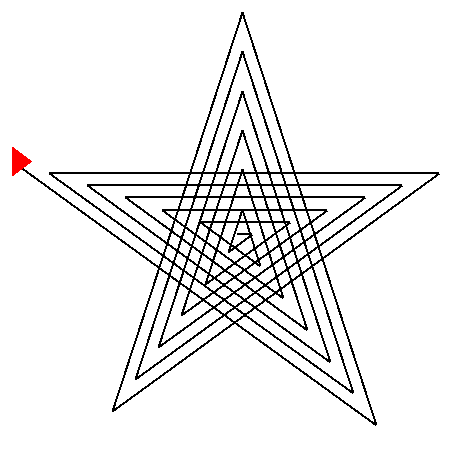
\includegraphics[width = 0.7\linewidth]{Star Spiral.png}
	\caption{A Star Spiral of 30 sides}
\end{figure}
\subsection{Peace}{\label{pp:peace}}
\textbf{Problem Statement:}\\
Draw the outline of the Proportionl Peace Sign according to measurements as shown in \ref{fig:peacemeasurements}.
\begin{figure}[H]
\centering
	\begin{subfigure}{\linewidth}
	\centering
	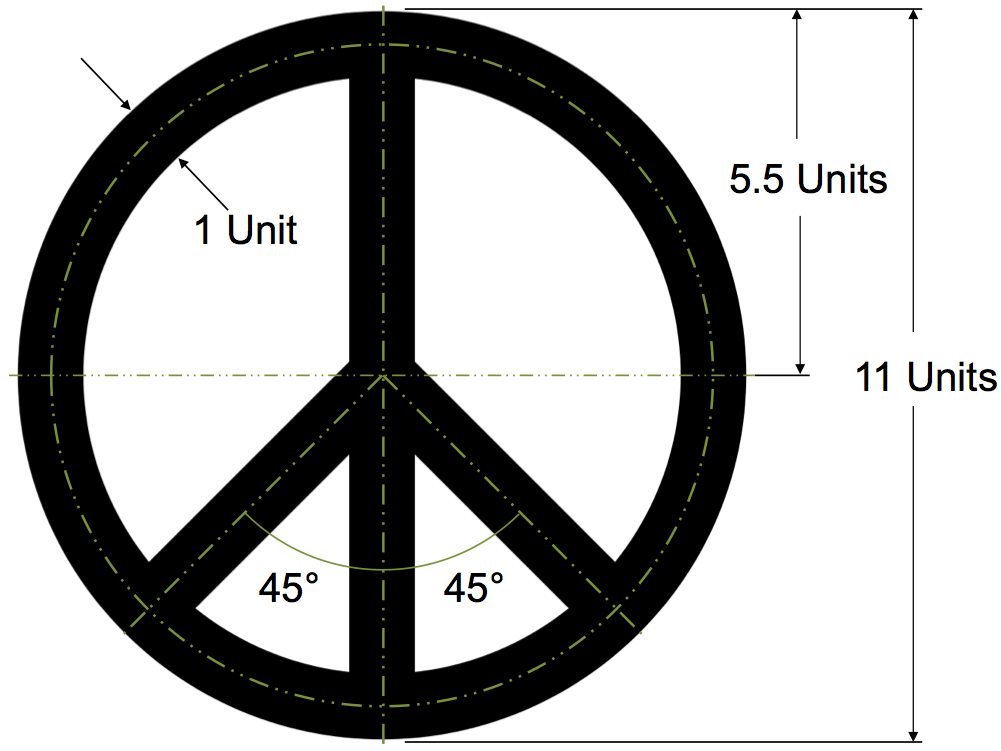
\includegraphics[width = 0.4\linewidth]{Peace Measurements.png}
	\caption{\href{https://bit.ly/peace-sign-measurements}{Measurements} by Jerry S. Sadin, based on (\href{https://bit.ly/peace-sign-wikipedia}{image} by \href{https://commons.wikimedia.org/wiki/User:SchuminWeb}{SchuminWeb})}
	\label{fig:peacemeasurements}
\end{subfigure}
\begin{subfigure}{\linewidth}
	\centering
	
\includegraphics[width = 0.65\linewidth]{Peace.png}
	\caption{Output generated using Simplecpp}
	\label{fig:peace}
\end{subfigure}
\caption{Peace Sign}
\end{figure}
The output image will look like \ref{fig:peace}.
\begin{funvideo}
\href{https://youtu.be/GO5FwsblpT8}{Carl Sagan's Pale Blue Dot -- carlsagandotcom}\\
\href{https://youtu.be/lshWT0iyxds}{Cosmos: Possible Worlds (Carl Sagan's Monologue) -- Evil Dead}
\end{funvideo}
\subsection{Butterfly}{\label{pp:butterfly}}
\textbf{Problem Statement:}\\
Print the Butterfly pattern for a general $n$. See Starter code (below) for more details.
\begin{testcases}
	{$t$ \hfill(number of test cases, an integer)\\
	$n_1\ n_2\ \ldots\ n_t$ \hfill($t$ space seperated integers for each testcase)}
	{Butterfly pattern \hfill(each test case on a newline)}
	{$1 \leq n_i \leq 10$}
	{5\\1 2 3 4 5}
	% {*\space\space\space*\newline*\space*\space*}
	{\vspace{-2em}
	\begin{figure}[H]
	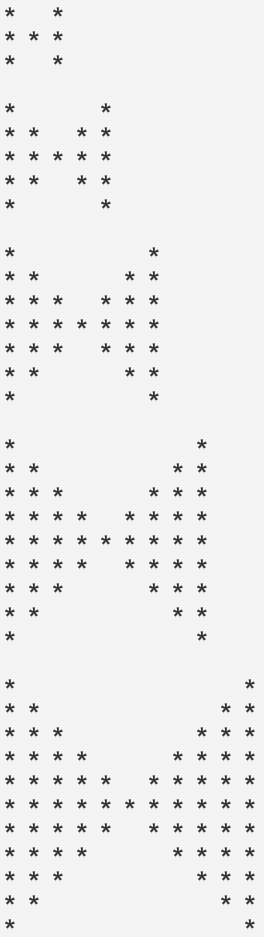
\includegraphics[width=0.23\linewidth]{Butterfly.png}
	\end{figure}
	}
	% \begin{table}[H]
	% \begin{tabular}{p{0.001pt}p{0.001pt}p{0.001pt}p{0.001pt}p{0.001pt}}
	% * &  &   &  & * \\
	% * &  & * &  & * \\
	% * &  &   &  & *
	% \end{tabular}
	% \end{table}
	% \begin{table}[H]
	% \begin{tabular}{lllll}
	% * &  &   &  & * \\
	% * &  & * &  & * \\
	% * &  &   &  & *
	% \end{tabular}
	% \end{table}
	{https://github.com/paramrathour/CS-101/tree/main/Starter Codes/Butterfly.cpp}
\end{testcases}
\begin{funvideo}
\href{https://youtu.be/fDek6cYijxI}{Chaos: The Science of the Butterfly Effect -- Veritasium}
\end{funvideo}
\subsection{Alphabetical Floyd's Triangle}{\label{pp:alphabeticalfloydstriangle}}
The alphabets are filled in alphabetical order (`A' to `Z') and a newline is started after printing $n$ alphabets on the $n$\textsuperscript{th} line. After `Z', the alphabets ``wrap around'' to `A'.

\textbf{Problem Statement:}\\
Print the left-aligned Alphabetical Floyd's Triangle for all given $n$. See Starter code (below) for more details.
\begin{testcases}
	{$t$ \hfill(number of test cases, an integer)\\$n_1\ n_2\ \ldots\ n_t$ \hfill($t$ space seperated integers for each testcase)}
	{Alphabetical Floyd's Triangle \hfill(left-aligned, each test case on a newline)}
	{$1 \leq n_i \leq 20$}
	{5\\1 2 3 5 17}
	{A\\[1em]A\\B C\\[1em]A\\B C\\D E F\\[1em]A\\B C\\D E F\\G H I J\\K L M N O\\[1em]A\\B C\\D E F\\G H I J\\K L M N O\\P Q R S T U\\V W X Y Z A B\\C D E F G H I J\\K L M N O P Q R S\\T U V W X Y Z A B C\\D E F G H I J K L M N\\O P Q R S T U V W X Y Z\\A B C D E F G H I J K L M\\N O P Q R S T U V W X Y Z A\\B C D E F G H I J K L M N O P\\Q R S T U V W X Y Z A B C D E F\\G H I J K L M N O P Q R S T U V W}
	{https://github.com/paramrathour/CS-101/tree/main/Starter Codes/Alphabetical Floyd's Triangle.cpp}
\end{testcases}
\subsection{Bernoulli's Triangle}{\label{pp:bernoullistriangle}}
You might have heard about \href{https://youtu.be/0iMtlus-afo}{Pascal's Triangle}. 
The $k$\textsuperscript{th} element of row $n$ of Bernoulli's Triangle is obtained by as shown in \ref{fig:bernoullistriangle} summing all elements of the row $n$ (row $0$ is the first row) until the $k$\textsuperscript{th} element (partial sums).
\begin{figure}[H]
	\centering
	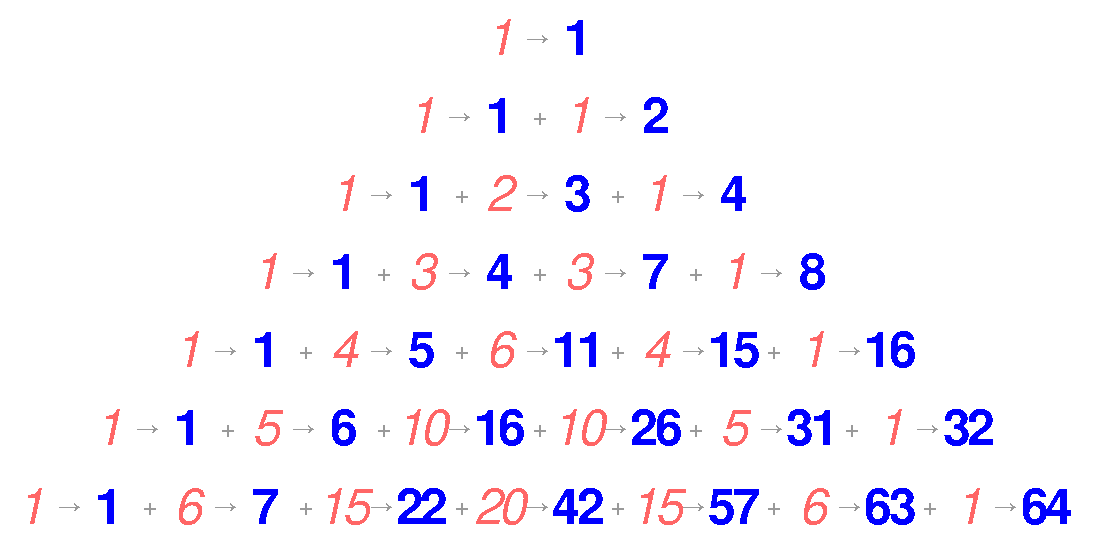
\includegraphics[width = 0.35\linewidth]{Bernoulli's Triangle.pdf}
	\caption{\textbf{\textcolor{blue}{Bernoulli's triangle}} from \textit{\textcolor{pink}{Pascal's triangle}} (\href{https://bit.ly/bernoullis-triangle}{Image} by \href{https://commons.wikimedia.org/wiki/User:Cmglee}{Cmglee} licensed under \href{https://creativecommons.org/licenses/by-sa/4.0/}{CC BY-SA 4.0})}
	% \caption{Bernoulli's triangle (\textbf{\textcolor{blue}{blue bold}} text) from Pascal's triangle (\textit{\textcolor{pink}{pink italics}}) (\href{https://bit.ly/bernoullis-triangle}{Image} by \href{https://commons.wikimedia.org/wiki/User:Cmglee}{Cmglee} licensed under \href{https://creativecommons.org/licenses/by-sa/4.0/}{CC BY-SA 4.0})}
	\label{fig:bernoullistriangle}
\end{figure}
% Formally given as below
% \begin{equation}
% B_{n,k} =  \sum _{p=0}^{k}{n \choose p}
% \end{equation}
\vspace{-1.5em}
\textbf{Problem Statement:}\\
Print the left-aligned Bernoulli's Triangle for all given $n$. See Starter code (below) for more details.
\begin{testcases}
	{$t$ \hfill(number of test cases, an integer)\\$n_1\ n_2\ \ldots\ n_t$ \hfill($t$ space seperated integers for each testcase)}
	{Bernoulli's Triangle \hfill(left-aligned, each test case on a newline)}
	{$0 \leq n_i \leq 20$}
	{4\\0 1 2 10}
	{1\\[1em]1\\1 2\\[1em]1\\1 2\\1 3 4\\[1em]1\\1 2\\1 3 4\\1 4 7 8\\1 5 11 15 16\\1 6 16 26 31 32\\1 7 22 42 57 63 64\\1 8 29 64 99 120 127 128\\1 9 37 93 163 219 247 255 256\\1 10 46 130 256 382 466 502 511 512\\1 11 56 176 386 638 848 968 1013 1023 1024}
	{https://github.com/paramrathour/CS-101/tree/main/Starter Codes/Bernoulli's Triangle.cpp}
\end{testcases}
\begin{funvideo}
\href{https://youtu.be/0iMtlus-afo}{Pascal's Triangle -- Numberphile}\\
\href{https://youtu.be/J0I1NuxUcpQ}{What You Don't Know About Pascal's Triangle -- Tipping Point Math}
\end{funvideo}
\KOMAoptions{paper=A3}
\recalctypearea
\subsection{Modular Times Table}{\label{pp:timestable}}
Procedure to construct the Modular Times Table:
\begin{itemize}
	\item Draw a circle which fits the entire ``drawing canvas''.
	\item Imagine you have $n$ equally-spaced points on the circumference of this circle. Number them $0$ to $n-1$ anti-clockwise with $0$ being the leftmost point.
	\item For each $i \in \{0,1,2,\ldots,n-1\}$ connect the points representing $i$ with the point for $(m\cdot i)\ \%\ n$ with a straight line.
\end{itemize} An example is shown in \ref{fig:timestable}. Don't draw the numbers. They are just to visualise the construction.
\begin{figure}[H]
	\centering
	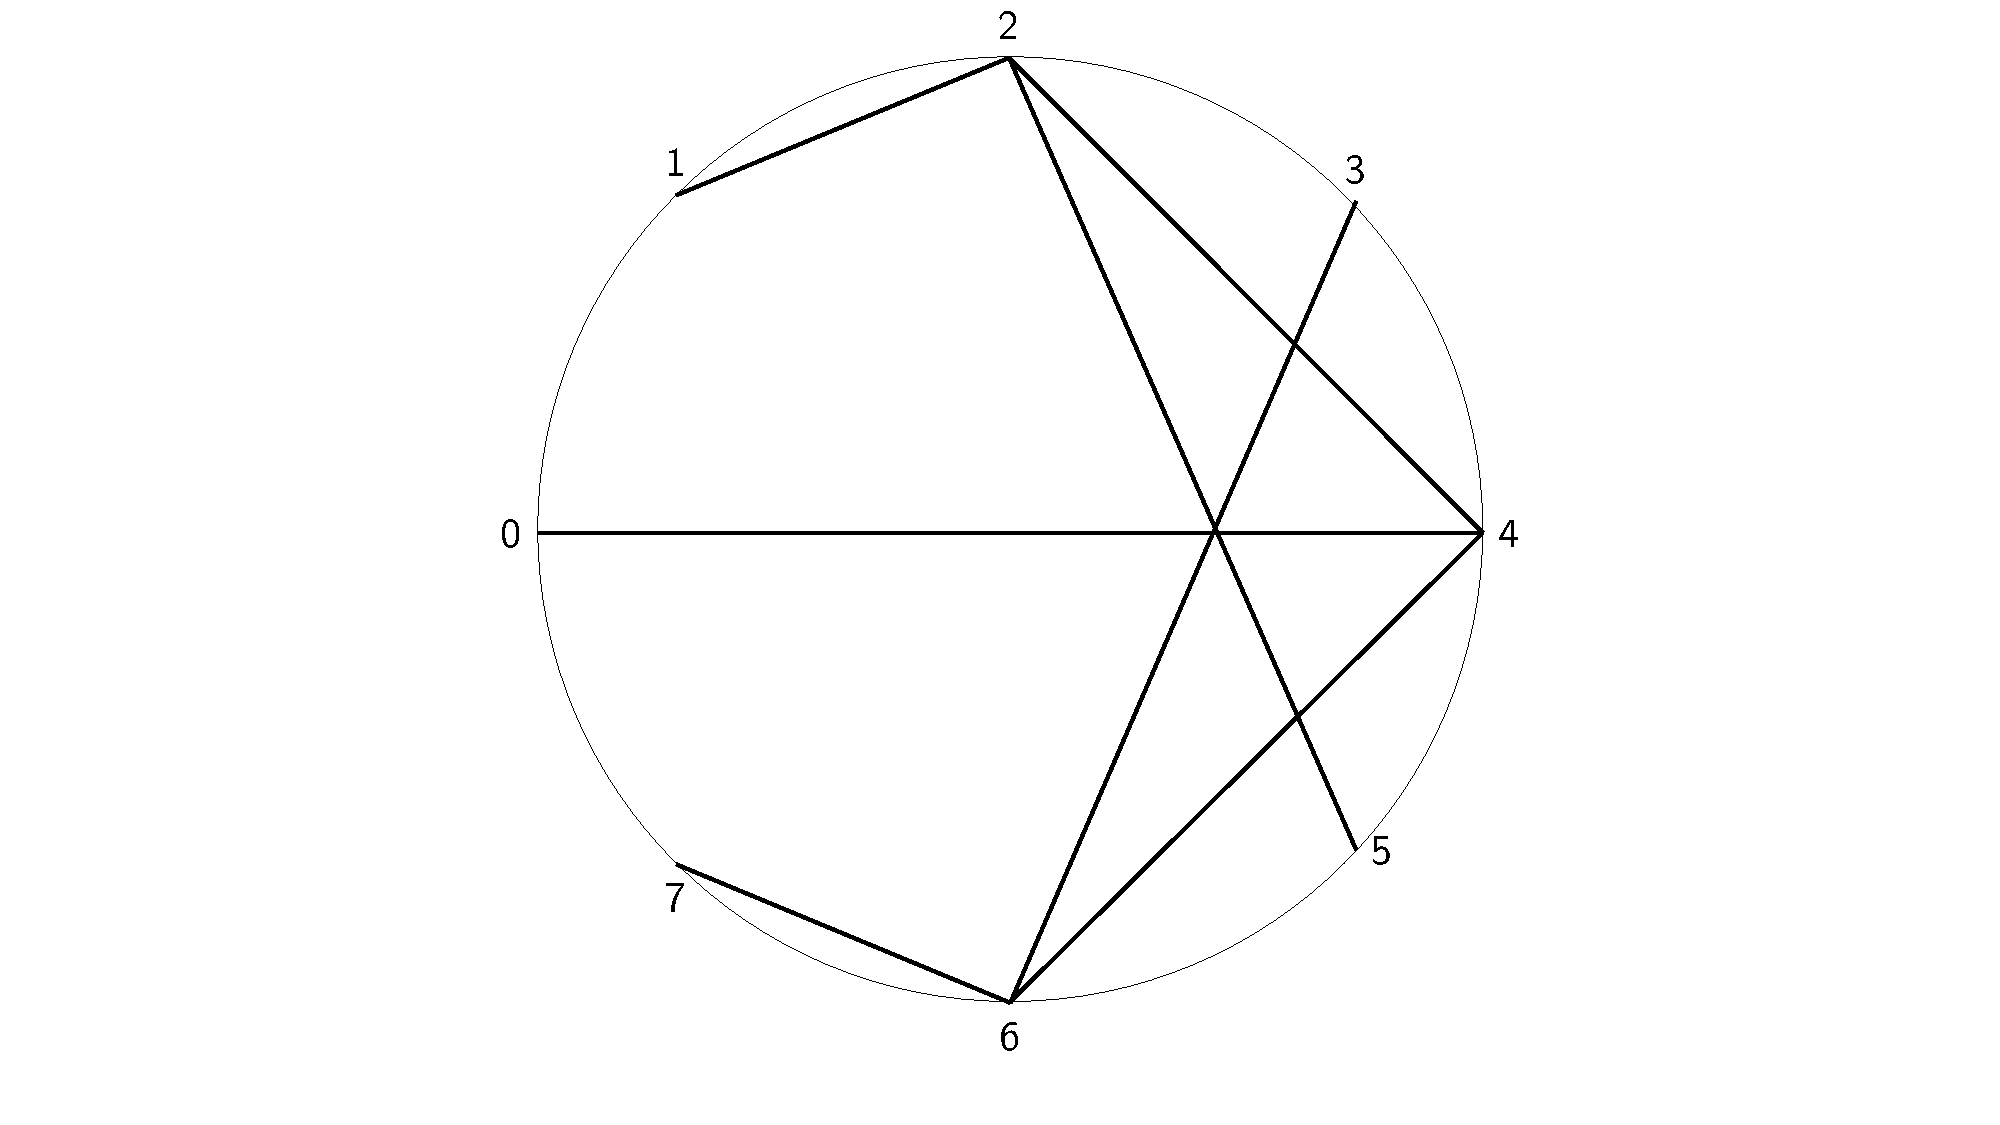
\includegraphics[width = 0.18\linewidth]{Modular Times Table.pdf}
	\caption{Times Table for $(n,m)=(8,2)$}
	\label{fig:timestable}
\end{figure}
\textbf{Problem Statement:}\\
For a given $(n,m)$ pair $(n>m)$, construct the Modular Times Table.
\begin{testcases}
	{$n\quad m$ \hfill(two numbers)}
	{The constructed Modular Times Table}
	{$3 \leq n \leq 500$\hfill(an integer)\\
	$1 < m < n$ \hfill(a double, first try to solve the problem for an integer $m$)}
	{See \ref{fig:timestabletestcases}}
	{See \ref{fig:timestabletestcases}}
	{https://github.com/paramrathour/CS-101/tree/main/Starter Codes/Modular Times Table.cpp}
\end{testcases}
\textbf{The output Modular Times Tables}
\begin{figure}[H]
	\centering
	\begin{subfigure}{0.145\linewidth}
		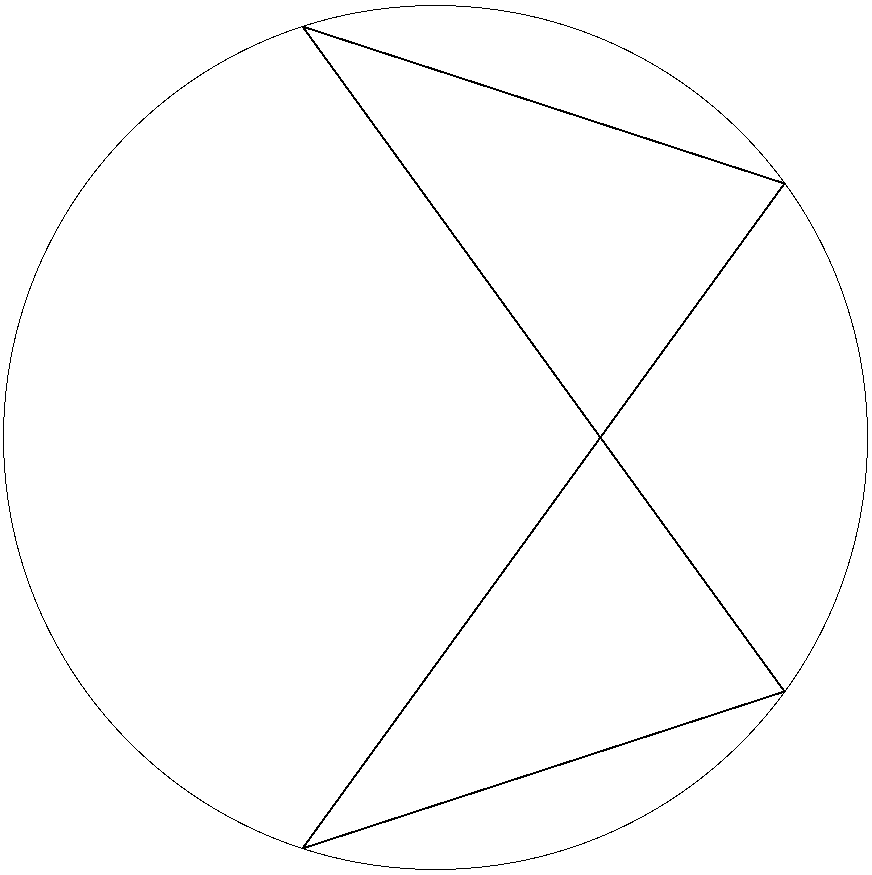
\includegraphics[width = \linewidth]{Modular Times Table/5 2.png}
		\caption{$(n,m) = (5,2)$}
	\end{subfigure}
	\begin{subfigure}{0.145\linewidth}
		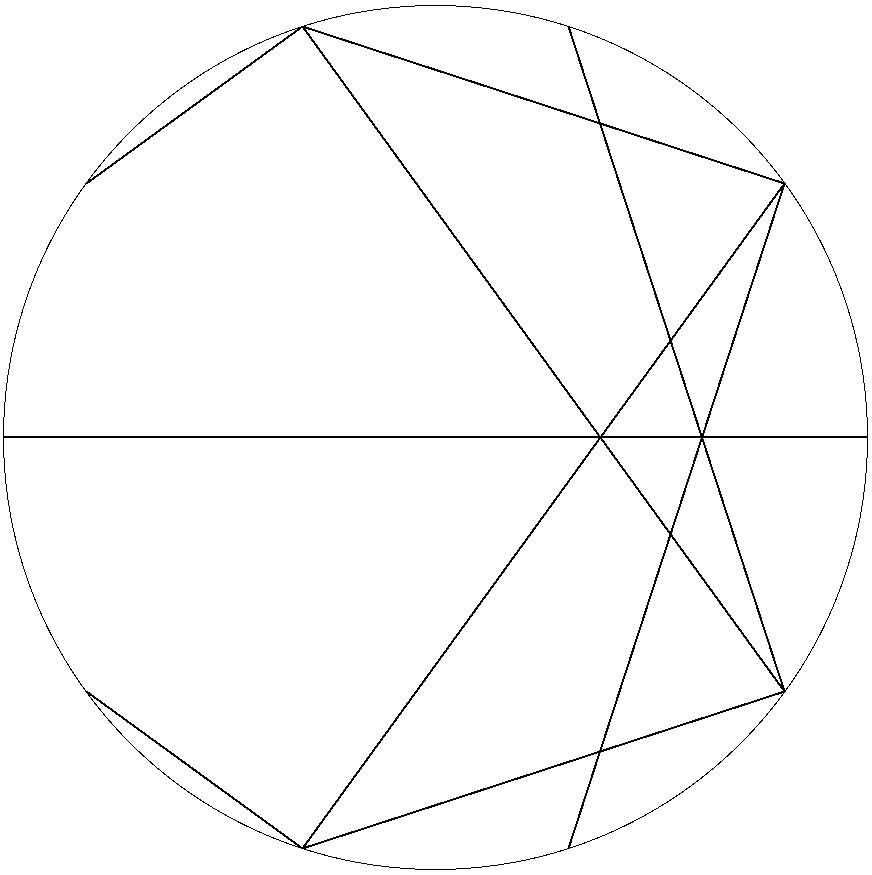
\includegraphics[width = \linewidth]{Modular Times Table/10 2.png}
		\caption{$(n,m) = (10,2)$}
	\end{subfigure}
	\begin{subfigure}{0.145\linewidth}
		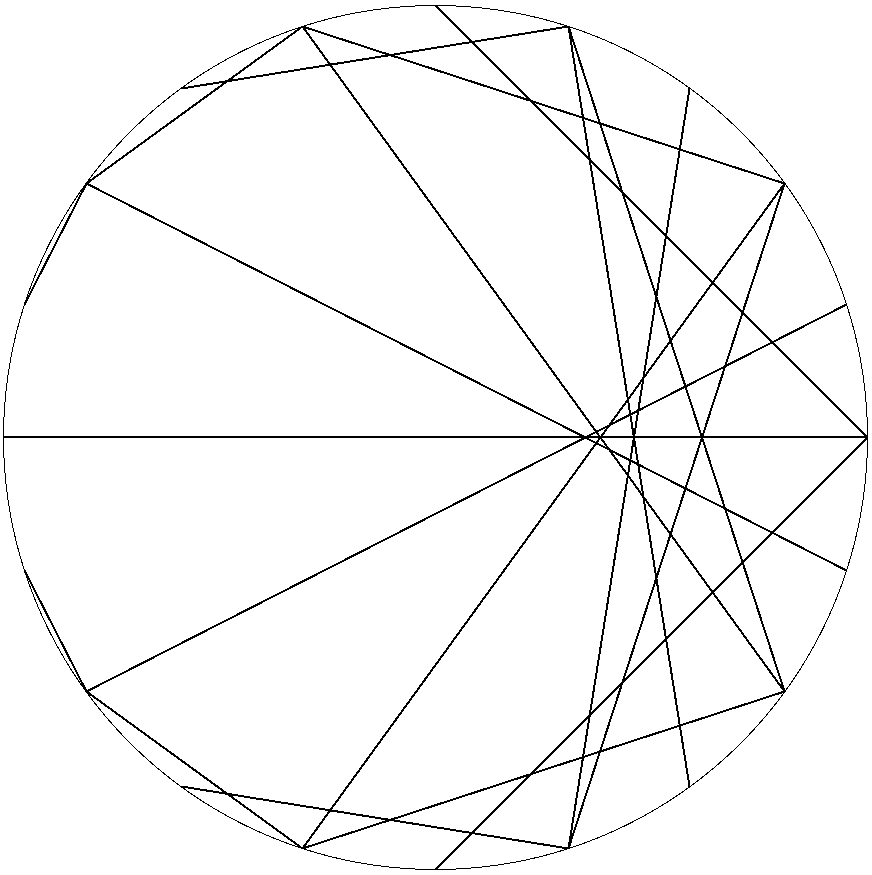
\includegraphics[width = \linewidth]{Modular Times Table/20 2.png}
		\caption{$(n,m) = (20,2)$}
	\end{subfigure}
	\begin{subfigure}{0.145\linewidth}
		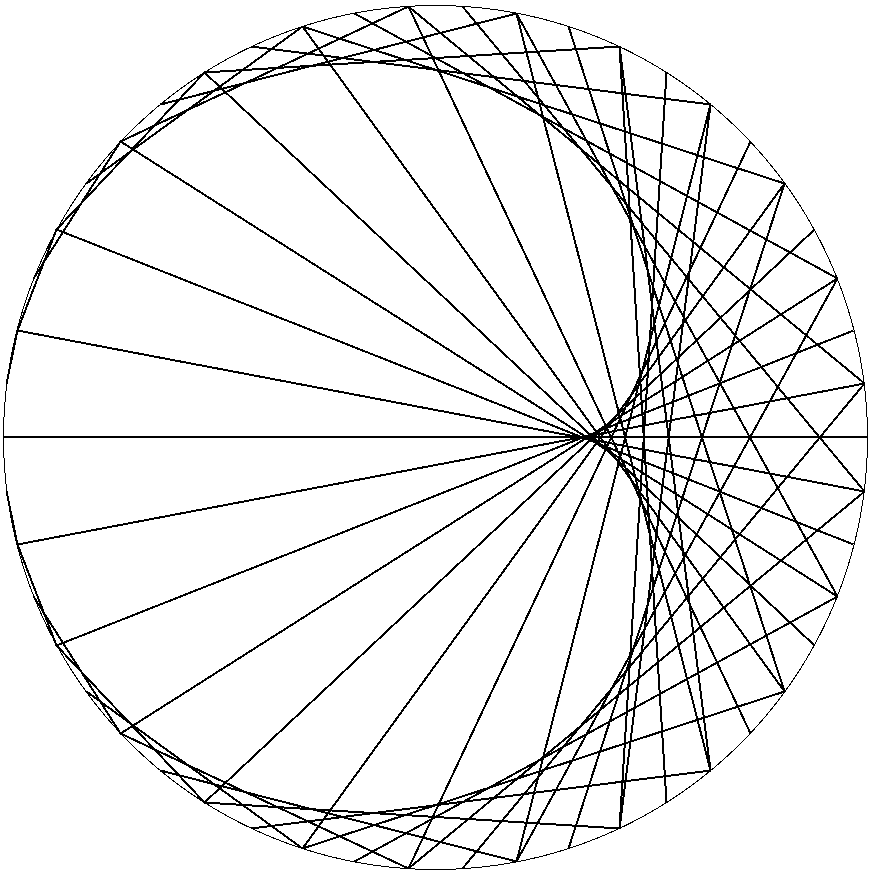
\includegraphics[width = \linewidth]{Modular Times Table/50 2.png}
		\caption{$(n,m) = (50,2)$}
	\end{subfigure}
	\begin{subfigure}{0.145\linewidth}
		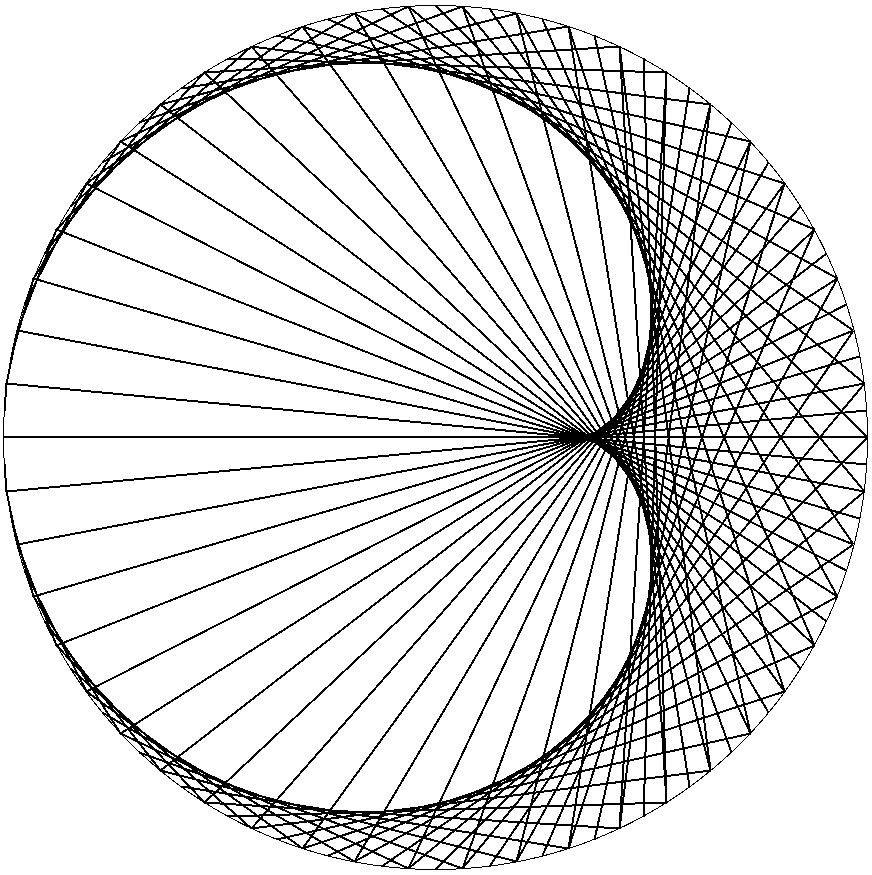
\includegraphics[width = \linewidth]{Modular Times Table/100 2.png}
		\caption{$(n,m) = (100,2)$}
	\end{subfigure}
	\begin{subfigure}{0.145\linewidth}
		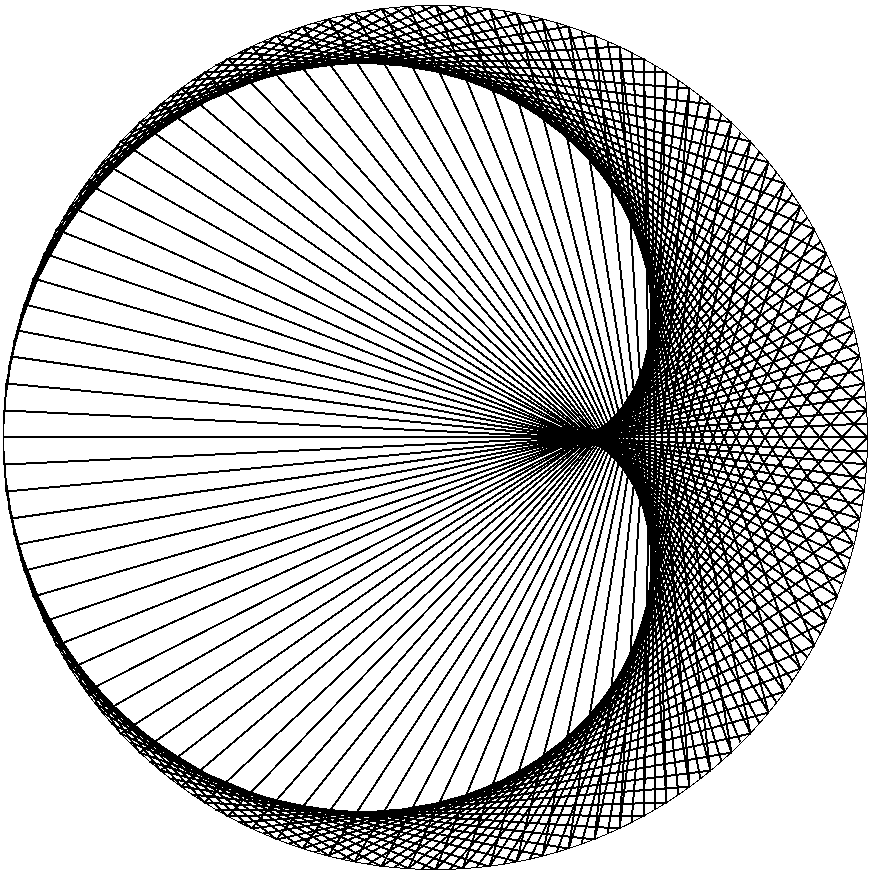
\includegraphics[width = \linewidth]{Modular Times Table/200 2.png}
		\caption{$(n,m) = (200,2)$}
	\end{subfigure}
		\begin{subfigure}{0.145\linewidth}
		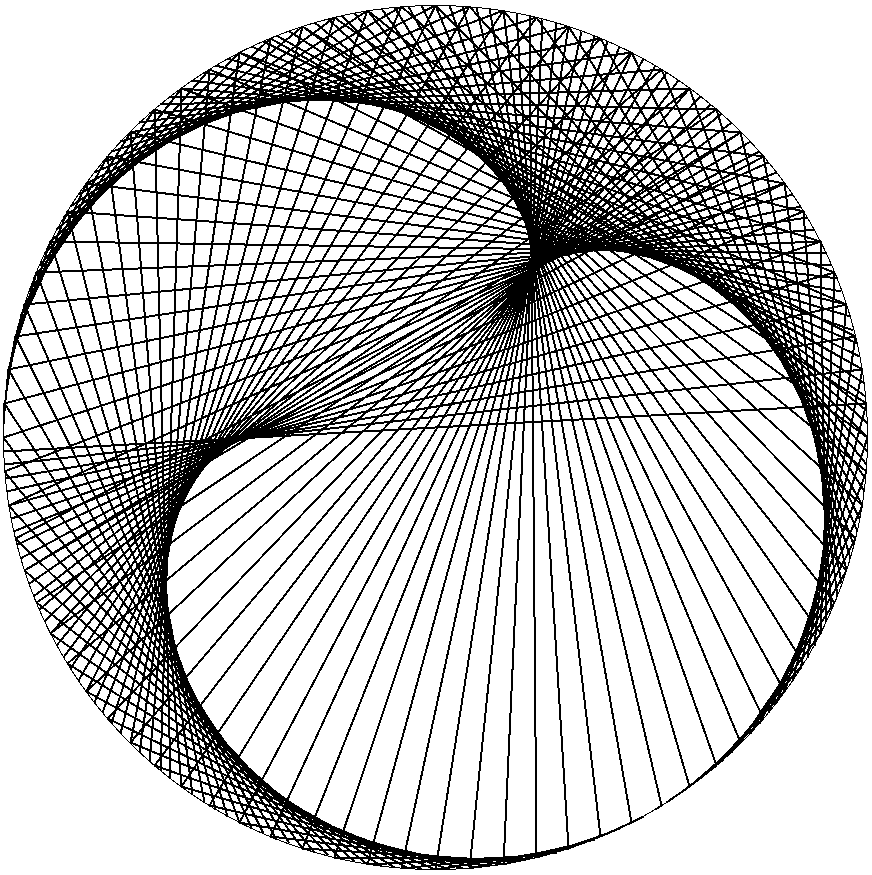
\includegraphics[width = \linewidth]{Modular Times Table/200 2.5.png}
		\caption{$(n,m) = (200,2.5)$}
	\end{subfigure}
	\begin{subfigure}{0.145\linewidth}
		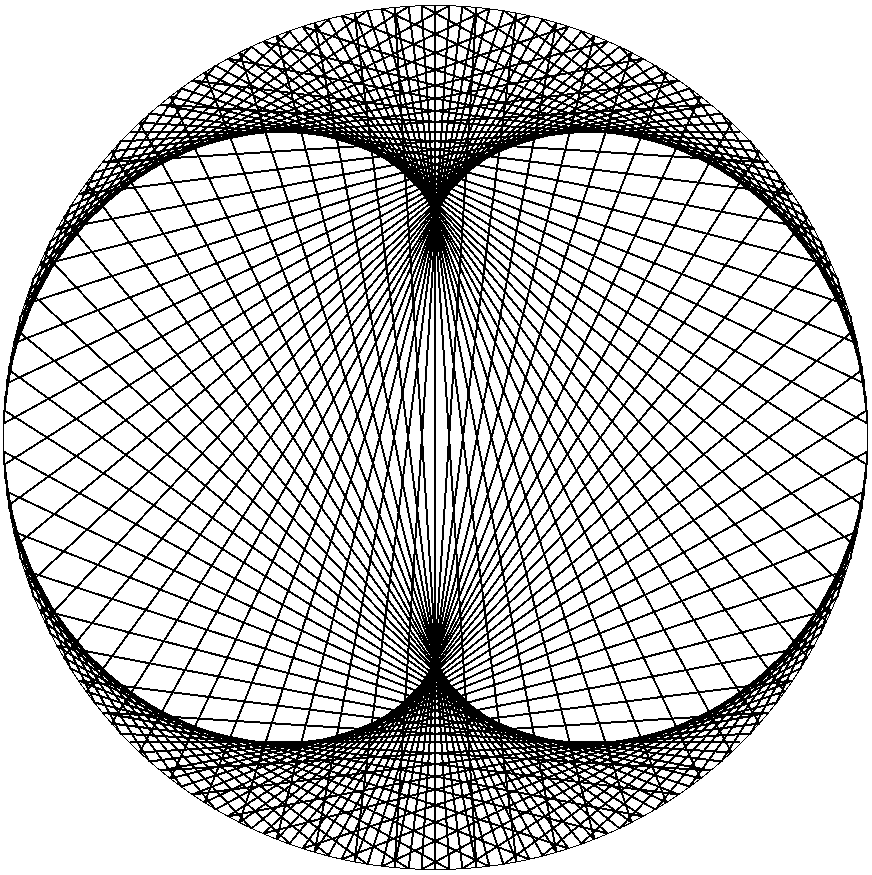
\includegraphics[width = \linewidth]{Modular Times Table/200 3.png}
		\caption{$(n,m) = (200,3)$}
	\end{subfigure}
	\begin{subfigure}{0.145\linewidth}
		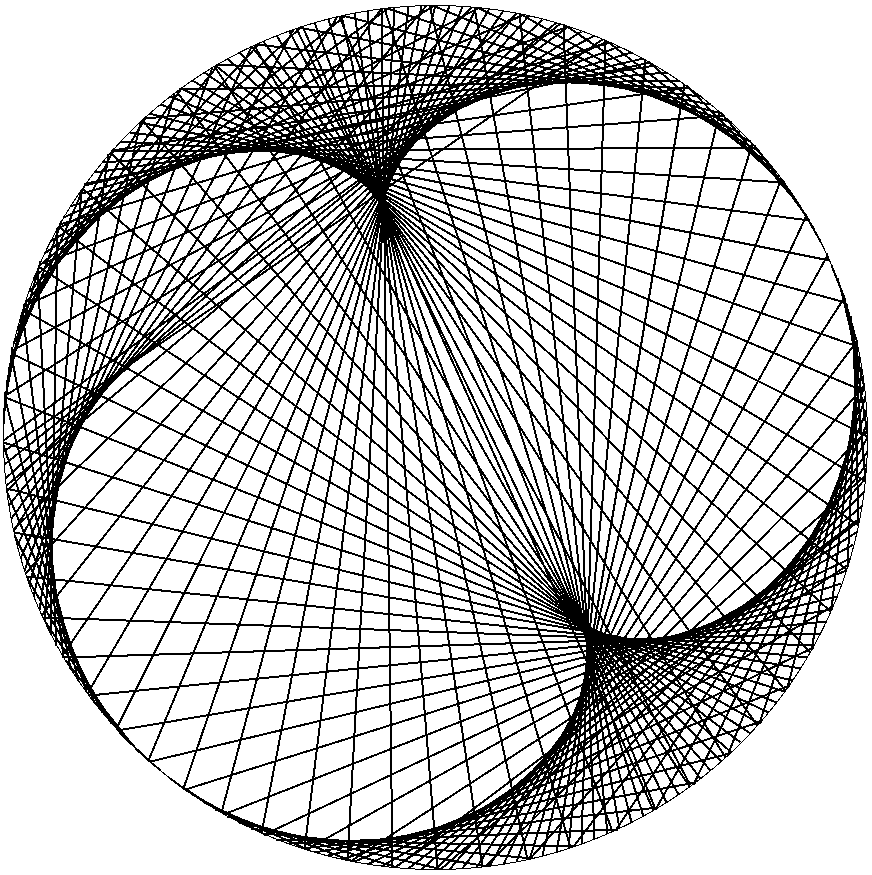
\includegraphics[width = \linewidth]{Modular Times Table/200 3.33.png}
		\caption{$(n,m) = (200,3.33)$}
	\end{subfigure}
	\begin{subfigure}{0.145\linewidth}
		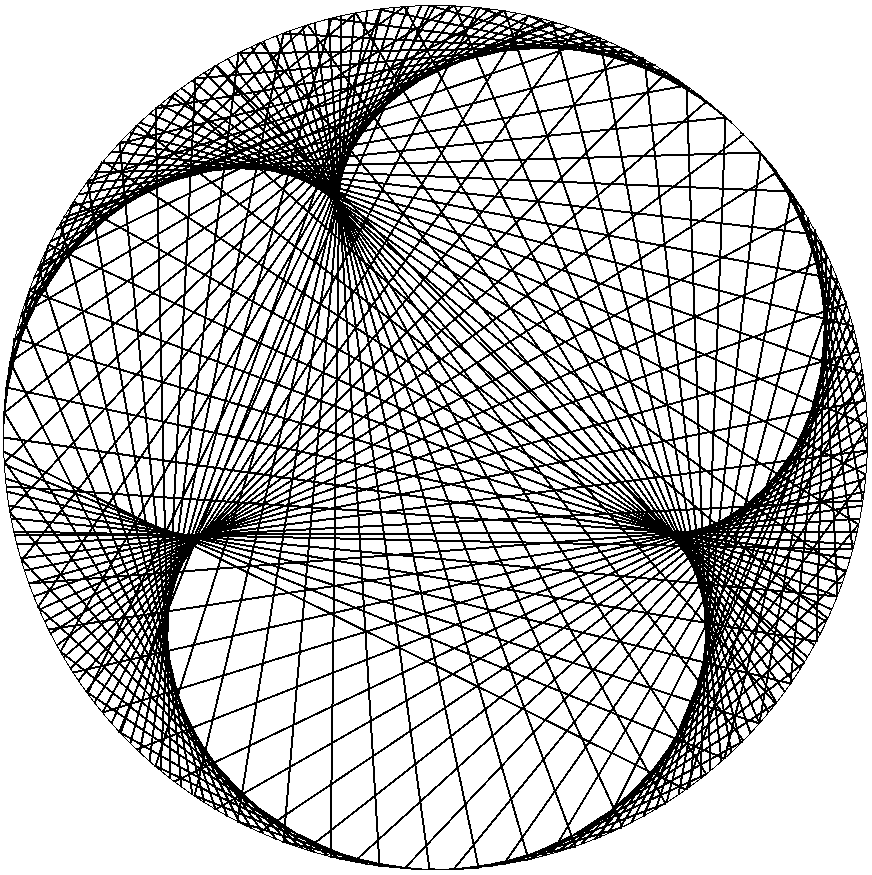
\includegraphics[width = \linewidth]{Modular Times Table/200 3.66.png}
		\caption{$(n,m) = (200,3.66)$}
	\end{subfigure}
	\begin{subfigure}{0.145\linewidth}
		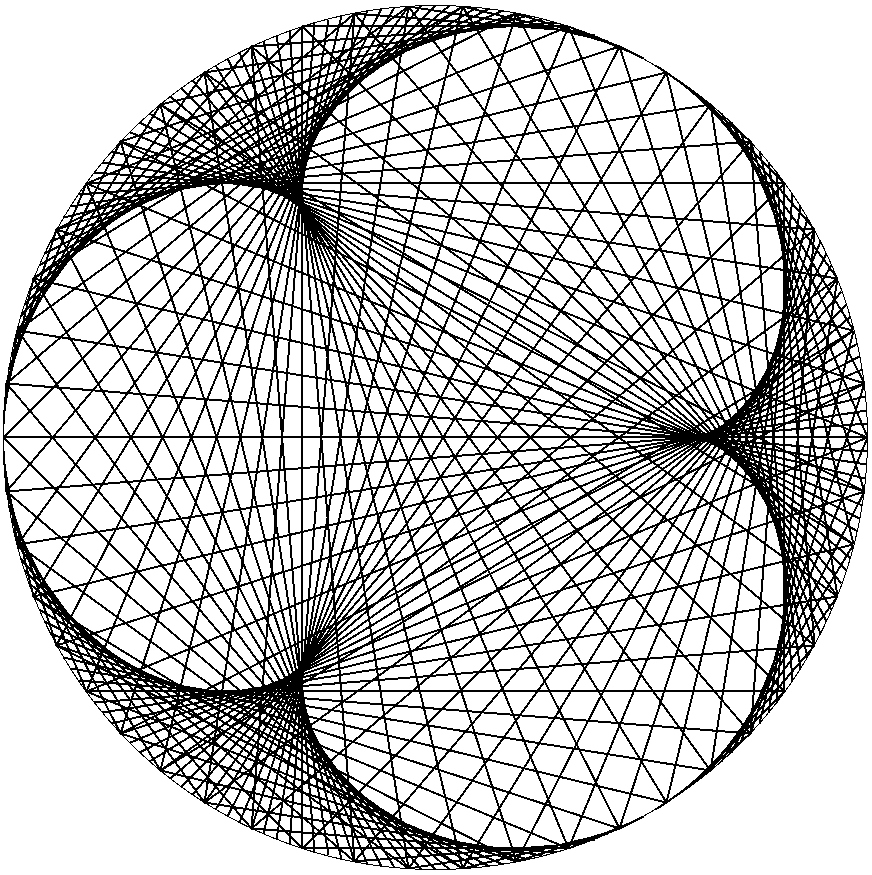
\includegraphics[width = \linewidth]{Modular Times Table/200 4.png}
		\caption{$(n,m) = (200,4)$}
	\end{subfigure}
	\begin{subfigure}{0.145\linewidth}
		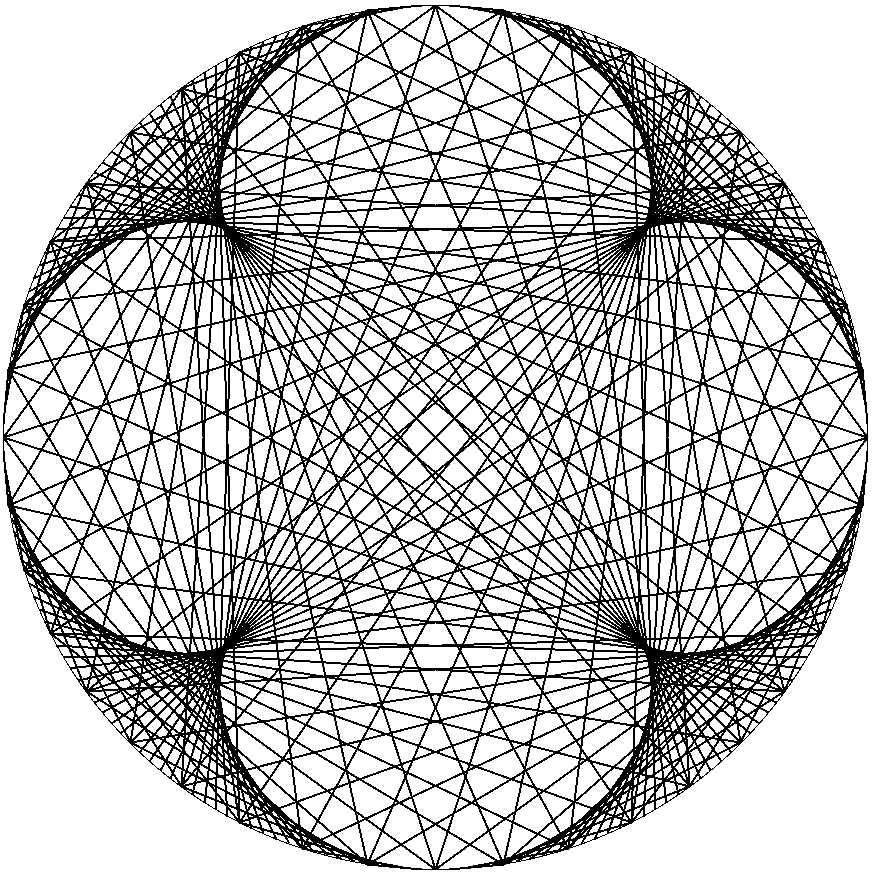
\includegraphics[width = \linewidth]{Modular Times Table/200 5.png}
		\caption{$(n,m) = (200,5)$}
	\end{subfigure}
	\begin{subfigure}{0.145\linewidth}
		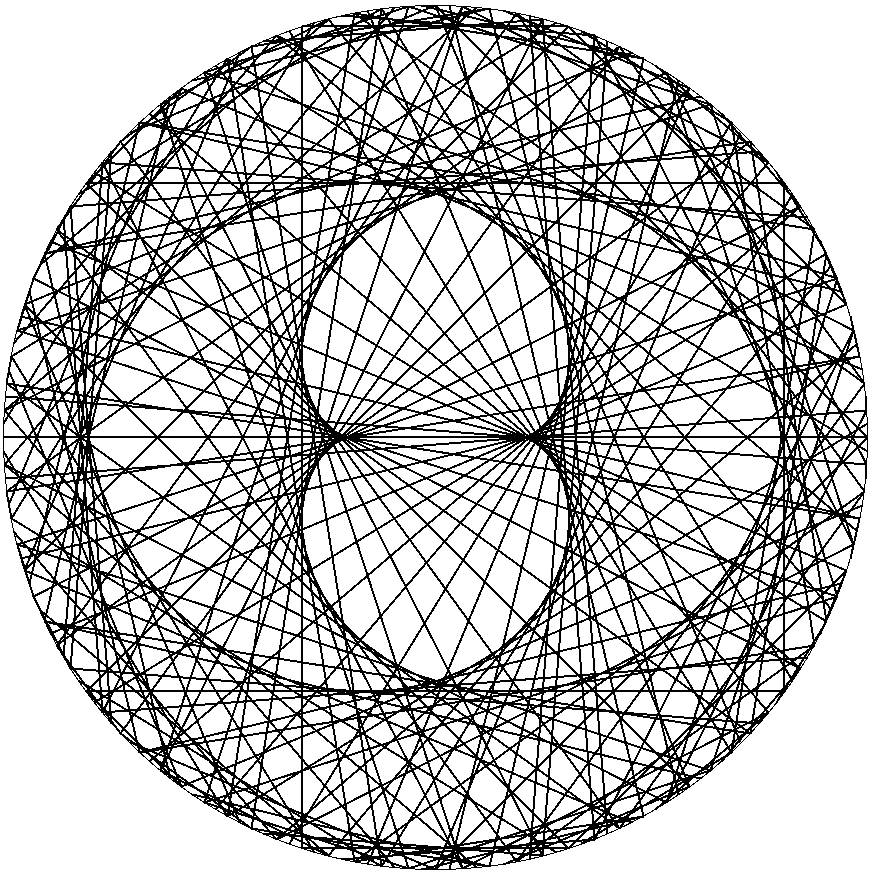
\includegraphics[width = \linewidth]{Modular Times Table/200 34.png}
		\caption{$(n,m) = (200,34)$}
	\end{subfigure}
	\begin{subfigure}{0.145\linewidth}
		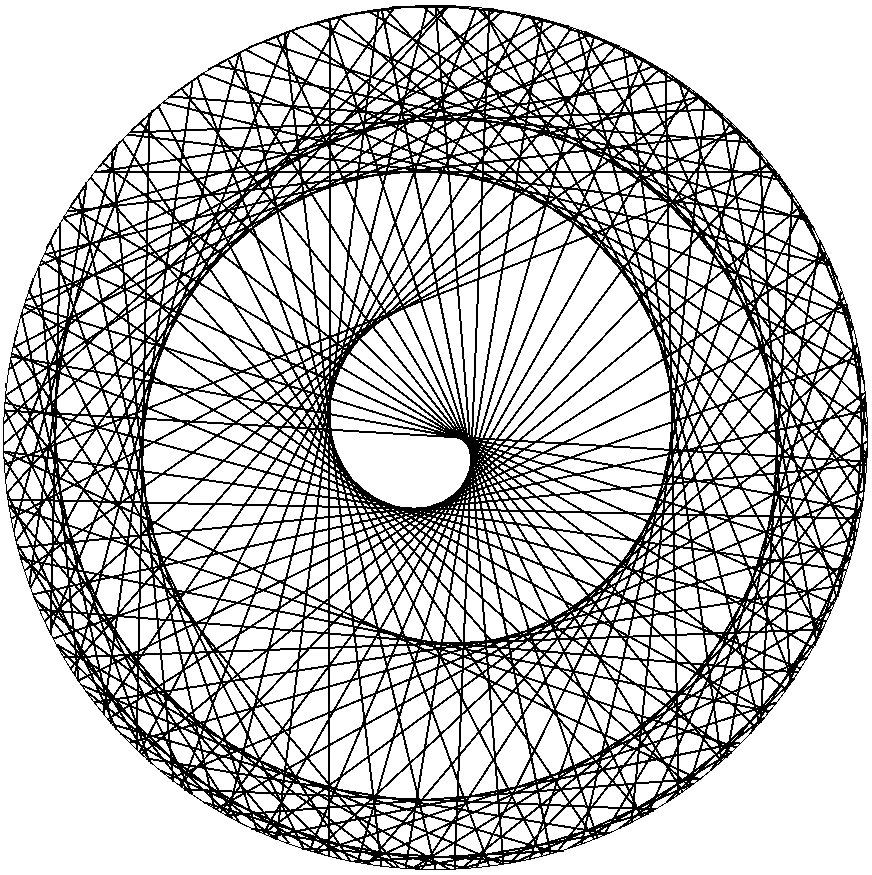
\includegraphics[width = \linewidth]{Modular Times Table/200 50.9.png}
		\caption{$(n,m) = (200,50.9)$}
	\end{subfigure}
	\begin{subfigure}{0.145\linewidth}
		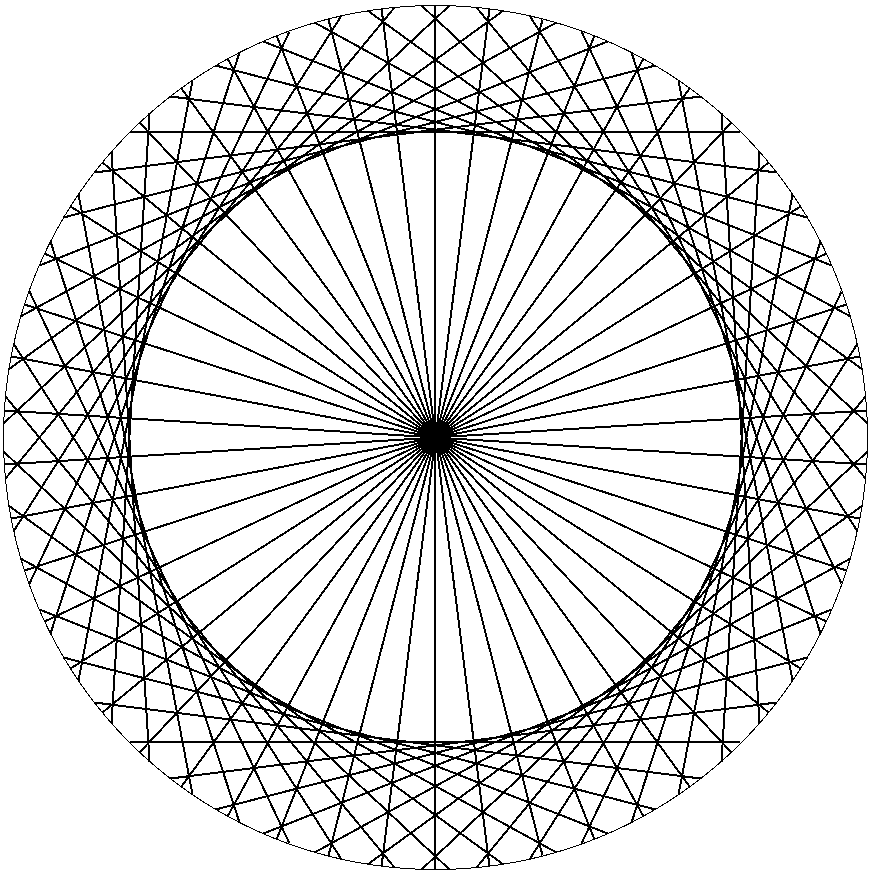
\includegraphics[width = \linewidth]{Modular Times Table/200 51.png}
		\caption{$(n,m) = (200,51)$}
	\end{subfigure}
	\begin{subfigure}{0.145\linewidth}
		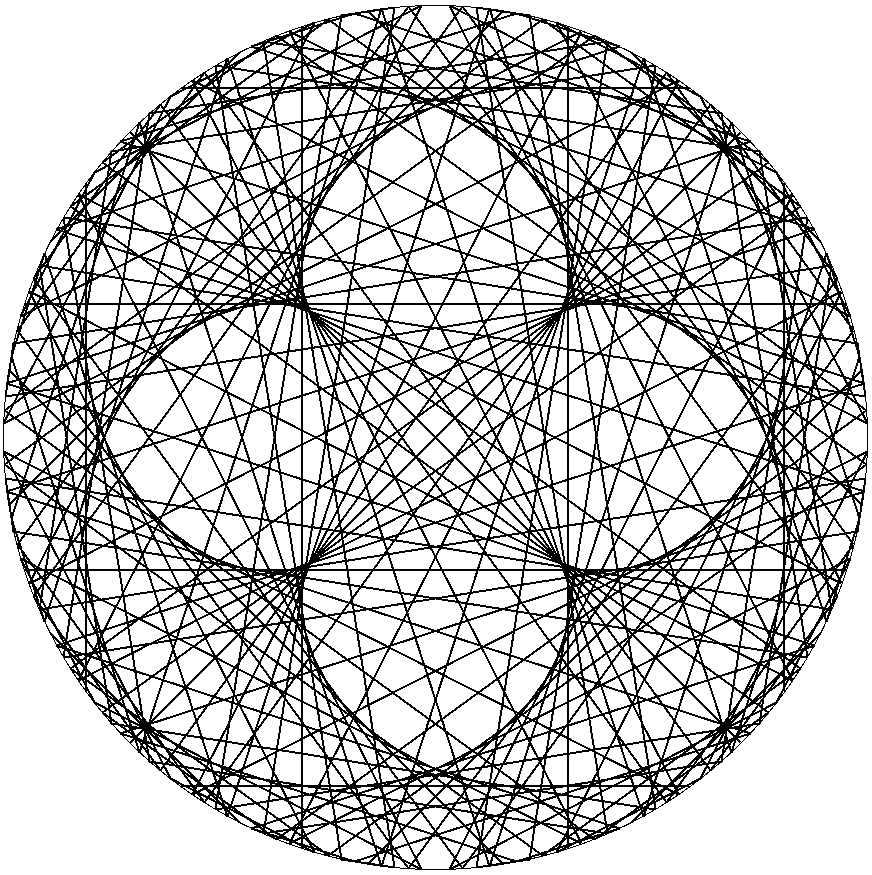
\includegraphics[width = \linewidth]{Modular Times Table/200 69.png}
		\caption{$(n,m) = (200,69)$}
	\end{subfigure}
	\begin{subfigure}{0.145\linewidth}
		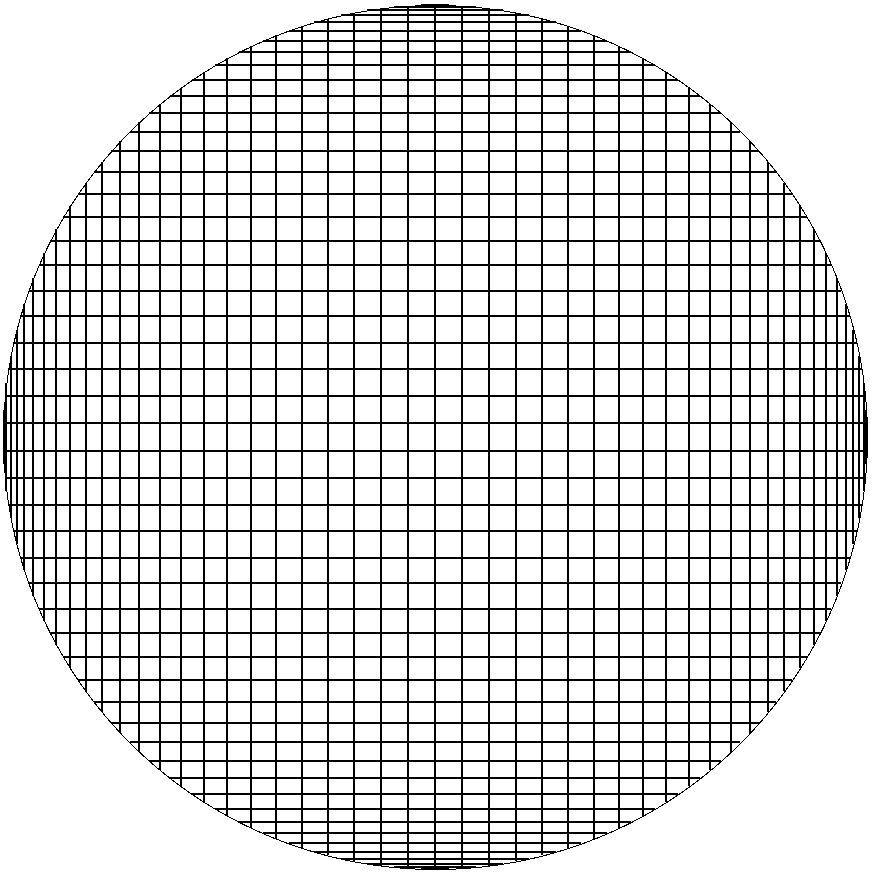
\includegraphics[width = \linewidth]{Modular Times Table/200 99.png}
		\caption{$(n,m) = (200,99)$}
	\end{subfigure}
	\begin{subfigure}{0.145\linewidth}
		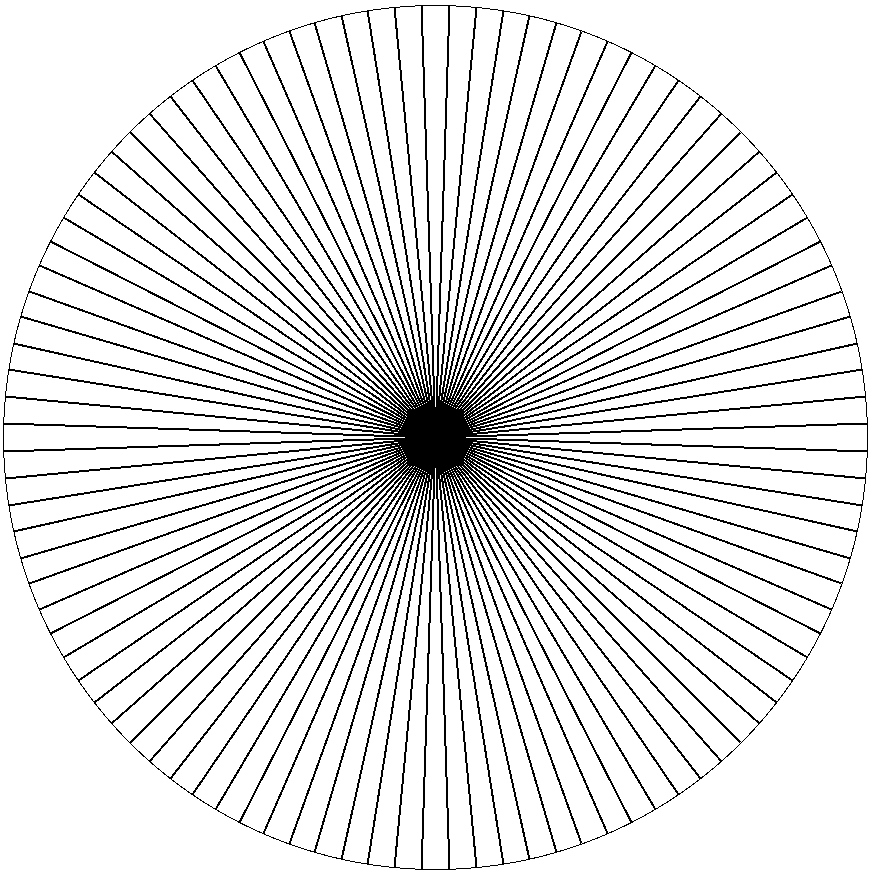
\includegraphics[width = \linewidth]{Modular Times Table/200 101.png}
		\caption{$(n,m) = (200,101)$}
	\end{subfigure}
	\caption{Modular Times Table}
	\label{fig:timestabletestcases}
\end{figure}
\begin{funvideo}
	\href{https://youtu.be/qhbuKbxJsk8}{Times Tables, Mandelbrot and the Heart of Mathematics}\\
	\href{https://www.geogebra.org/m/z8wrdret}{Modular Times Tables}
\end{funvideo}
\KOMAoptions{paper=A4}
\recalctypearea